%%%%%%%%%%%%%%%%%%%%%%%%%%%%%%%%%%%%%
%                                   %
% Compile with XeLaTeX and biber    %
%                                   %
% Questions or comments:            %
%                                   %
% joshua dot mcneill at uga dot edu %
%                                   %
%%%%%%%%%%%%%%%%%%%%%%%%%%%%%%%%%%%%%

\documentclass{beamer}
  % Read in standard preamble (cosmetic stuff)
  %%%%%%%%%%%%%%%%%%%%%%%%%%%%%%%%%%%%%%%%%%%%%%%%%%%%%%%%%%%%%%%%
% This is a standard preamble used in for all slide documents. %
% It basically contains cosmetic settings.                     %
%                                                              %
% Joshua McNeill                                               %
% joshua dot mcneill at uga dot edu                            %
%%%%%%%%%%%%%%%%%%%%%%%%%%%%%%%%%%%%%%%%%%%%%%%%%%%%%%%%%%%%%%%%

% Beamer settings
% \usetheme{Berkeley}
\usetheme{CambridgeUS}
% \usecolortheme{dove}
% \usecolortheme{rose}
\usecolortheme{seagull}
\usefonttheme{professionalfonts}
\usefonttheme{serif}
\setbeamertemplate{bibliography item}{}

% Packages and settings
\usepackage{fontspec}
  \setmainfont{Charis SIL}
\usepackage{hyperref}
  \hypersetup{colorlinks=true,
              allcolors=blue}
\usepackage{graphicx}
  \graphicspath{{../../figures/}}
\usepackage[normalem]{ulem}
\usepackage{enumerate}

% Document information
\author{M. McNeill}
\title[FREN2001]{Français 2001}
\institute{\url{joshua.mcneill@uga.edu}}
\date{}

%% Custom commands
% Lexical items
\newcommand{\lexi}[1]{\textit{#1}}
% Gloss
\newcommand{\gloss}[1]{`#1'}
\newcommand{\tinygloss}[1]{{\tiny`#1'}}
% Orthographic representations
\newcommand{\orth}[1]{$\langle$#1$\rangle$}
% Utterances (pragmatics)
\newcommand{\uttr}[1]{`#1'}
% Sentences (pragmatics)
\newcommand{\sent}[1]{\textit{#1}}
% Base dir for definitions
\newcommand{\defs}{../definitions}


  % Packages and settings

  % Document information
  \subtitle[Révision, examen 1]{Révision pour l'examen 1}

\begin{document}
  % Read in the standard intro slides (title page and table of contents)
  \begin{frame}
    \titlepage
    \tiny{Office: % Basically a variable for office hours location
Gilbert 121\\
          Office hours: % Basically a variable for office hours
 lundi, mercredi, vendredi 10:10--11:10
}
  \end{frame}

  \begin{frame}{Choose Your Own Adventure}
    \hypertarget{début}{}
    \begin{columns}
      \column{0.5\textwidth}
        \begin{center}
          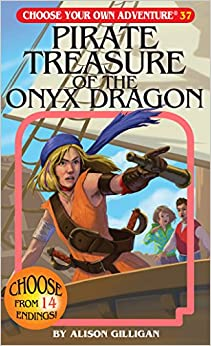
\includegraphics[scale=0.5]{aventure.jpg} \\
          Le Trésor de pirate du dragon d'onyx
        \end{center}
      \column{0.5\textwidth}
        Tu es sur un bateau.
        Tu sens ...
        \begin{enumerate}
          \item \hyperlink{questions}{des questions} au nord.
          \item \hyperlink{passé}{le passé} à l'est.
          \item \hyperlink{pronoms}{des pronoms} au sud.
          \item \hyperlink{modes}{des modes} à l'ouest.
        \end{enumerate}
        Choisis une direction.
    \end{columns}
  \end{frame}

  \begin{frame}{Questions}
    \hypertarget{questions}{}
    \begin{columns}
      \column{0.5\textwidth}
        Tu trouves un vaisseau fantôme dans un orage.
        Tu décides de poser des questions au capitaine.
        Tu peux utiliser ...
        \begin{enumerate}
          \item les mots \hyperlink{que}{\lexi{qui} et \lexi{que}}.
          \item le mot \hyperlink{quel}{\lexi{quel/le/s}}.
        \end{enumerate}
        Ou tu peux retourner \hyperlink{début}{au sud} si tu as peur...
      \column{0.5\textwidth}
        \begin{center}
          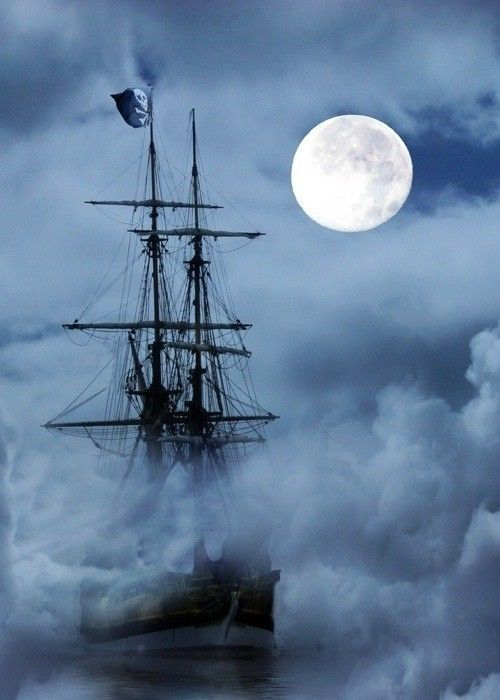
\includegraphics[scale=0.27]{vaisseau.jpg}
        \end{center}
    \end{columns}
  \end{frame}

  \begin{frame}{\lexi{Qui} et \lexi{que}}
    \hypertarget{que}{}
    Il répond à tes questions.
    Qu'est-ce que tu lui demandes?
    \begin{enumerate}
      \item Le week-end, je fais \underline{du surf}.
      \item<2->[$\to$] Qu'est-ce que tu fais le week-end?
      \item<3-> Je fais du surf avec \underline{ma sœur}.
      \item<4->[$\to$] Avec qui fais-tu du surf?
      \item<5-> Je vois \underline{Pam} sur la plage.
      \item<6->[$\to$] Qui est-ce que tu vois sur la plage?
      \item<7-> \underline{De la plongée} se passe.
      \item<8->[$\to$] Qu'est-ce qui se passe?
    \end{enumerate}
    Tu peux lui poser des questions avec \hyperlink{quel}{\lexi{quel/le/s}} ou retourner \hyperlink{début}{au sud}.
  \end{frame}

  \begin{frame}{\lexi{Quel/le/s}}
    \hypertarget{quel}{}
    Il répond à tes questions.
    Quelle version du mot \lexi{quel/le/s} utilises-tu?
    \begin{enumerate}
      \item \underline{\uncover<2->{Quel}} est ton préféré, un jardin ou un potager?
      \item[$\to$] Je préfère un jardin, parce que je ne mange pas.
      \item<3-> Tu mets un jardin près de \underline{\uncover<4->{quelle}} rivière?
      \item<3->[$\to$] Il ne faut pas le mettre près d'une rivière.
      \item<5-> \underline{\uncover<6->{Quels}} endroits sont les meilleurs?
      \item<5->[$\to$] Un champ ou une vallée, peut-être. Je ne sais pas; je suis un fantôme.
    \end{enumerate}
    Tu peux lui poser des questions avec \hyperlink{que}{\lexi{qui} et \lexi{que}} ou retourner \hyperlink{début}{au sud}.
  \end{frame}

  \begin{frame}{Passé}
    \hypertarget{passé}{}
    \begin{columns}
      \column{0.5\textwidth}
        Tu te trouves sur une île inhabitée.
        Dans le sable, tu vois des leçons de grammaire.
        Tu peux examiner ...
        \begin{enumerate}
          \item \hyperlink{composé}{le passé composé}.
          \item \hyperlink{imparfait}{l'imparfait}.
          \item \hyperlink{simple}{le passé simple}.
        \end{enumerate}
        Ou si tu as de la chance, tu peux construire un canoë et retourner \hyperlink{mort}{à l'ouest}...
      \column{0.5\textwidth}
        \begin{center}
          \includegraphics[scale=0.13]{inhabitée.jpg}
        \end{center}
    \end{columns}
  \end{frame}

  \begin{frame}{Imparfait}
    \hypertarget{imparfait}{}
    Ce sont simplement des phrases insensées.
    \begin{enumerate}
      \item Il \underline{\uncover<2->{faisait}} (was) 87 degrés avant-hier.
      \item<3-> Les chats \underline{\uncover<4->{maigrissaient}} (were getting skinny).
      \item<5-> Nous \underline{\uncover<6->{prenions}} (would take) l'ascenseur tous les jours.
      \item<7-> Quelquefois, vous \underline{\uncover<8->{alliez}} (would go) à l'armoire pour choisir des vêtements.
    \end{enumerate}
    Ces phrases sont inutiles, donc tu décides d'\hyperlink{passé}{examiner une autre leçon}.
  \end{frame}

  \begin{frame}{Passé composé}
    \hypertarget{composé}{}
    C'est une histoire de la dernière personne sur l'île: Mack.
    \begin{enumerate}
      \item Mack \underline{\uncover<2->{est allé}} (went) à la pêche.
      \item<3-> Des poissons du lac \underline{\uncover<4->{sont arrivés}} (arrived).
      \item<5-> Il les \underline{\uncover<6->{a pris}} (caught),
      \item<7-> et il \underline{\uncover<8->{a fait}} (made) des skis nautiques des poissons.
    \end{enumerate}
    Ça semble improbable, donc tu décides d'\hyperlink{passé}{examiner une autre leçon}.
  \end{frame}

  \begin{frame}{Passé simple}
    \hypertarget{simple}{}
    Tu ne \alert{pus} pas comprendre la leçon, parce que tu n'as pas encore appris le passé simple.
    Tu décides d'\hyperlink{passé}{examiner une autre leçon}.
  \end{frame}

  \begin{frame}{Pronoms}
    \hypertarget{pronoms}{}
    \begin{columns}
      \column{0.5\textwidth}
        Il y a un monstre de mer.
        Tu le vois, et tu réfléchis à l'attaquer.
        Tu peux l'attaquer avec ...
        \begin{enumerate}
          \item \hyperlink{direct}{des objets directs}.
          \item \hyperlink{indirect}{des objets indirects}.
          \item \hyperlink{y}{le pronom \lexi{y}}.
        \end{enumerate}
        Ou tu peux retourner \hyperlink{début}{au nord} si tu as peur...
      \column{0.5\textwidth}
        \begin{center}
          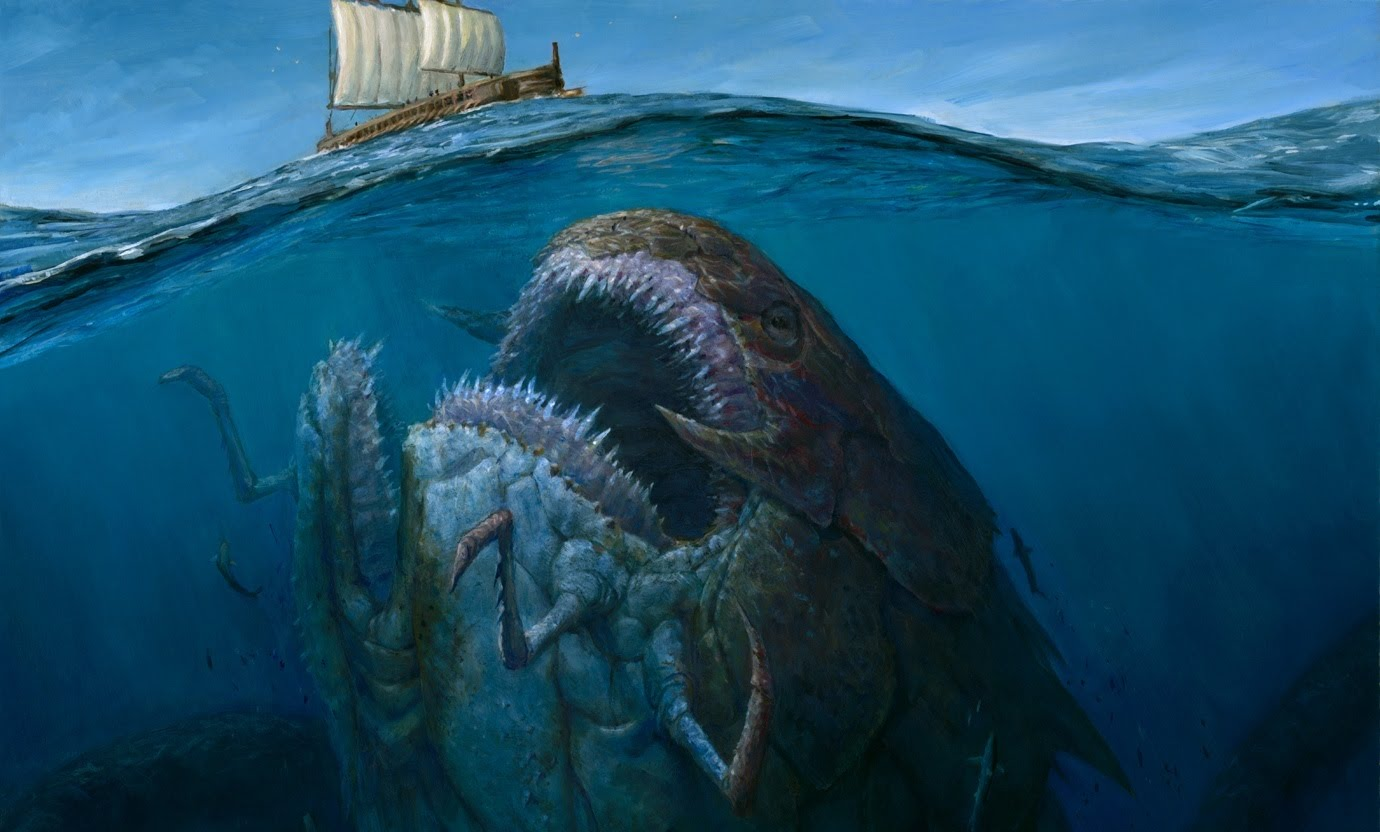
\includegraphics[scale=0.12]{monstre.jpg}
        \end{center}
    \end{columns}
  \end{frame}

  \begin{frame}{Objets directs}
    \hypertarget{direct}{}
    \begin{enumerate}
      \item Ron loue \alert<2->{le studio} à son ami.
      \item<3->[$\to$] Ron \alert{le} loue à son ami.
      \item<4-> Allison prête \alert<5->{l'étagère} à Ron.
      \item<6->[$\to$] Allison \alert{la} prête à Ron.
      \item<7-> Ils ont emprunté \alert<8->{les fauteuils dans le séjour}.
      \item<9->[$\to$] Ils \alert{les} ont emprunté\alert{s}.
    \end{enumerate}
    Tu fais mal \gloss{hurt} au monstre avec tes compétences dans les objets directs, mais il n'est pas mort.
    Il faut l'attaquer avec \hyperlink{pronoms}{quelque chose d'autre}.
  \end{frame}

  \begin{frame}{Objets indirects}
    \hypertarget{indirect}{}
    \begin{enumerate}
      \item Sandra offre la plante \alert<2->{à l'infirmière}.
      \item<3->[$\to$] Sandra \alert{lui} offre la plante.
      \item<4-> Le chanteur écrit une lettre \alert<5->{au pharmacien}.
      \item<6->[$\to$] Le chanteur \alert{lui} écrit une lettre.
      \item<7-> L'avocat a apporté les photos \alert<8->{aux architectes}.
      \item<9->[$\to$] L'avocat \alert{leur} a apporté les photos.
    \end{enumerate}
    Tu fais mal \gloss{hurt} au monstre avec tes compétences dans les objets indirects, mais il n'est pas mort.
    Il faut l'attaquer avec \hyperlink{pronoms}{quelque chose d'autre}.
  \end{frame}

  \begin{frame}{\lexi{Y}}
    \hypertarget{y}{}
    Tu prends le pronom \lexi{y}, mais tu te tires dans le pied \gloss{shoot yourself in the foot}, parce que tu n'as pas encore appris le pronom \lexi{y}.
    Le monstre te mange.
    Tu es \hyperlink{mort}{mort/e}.
  \end{frame}

  \begin{frame}{Modes}
    \hypertarget{modes}{}
    \begin{columns}
      \column{0.5\textwidth}
        Tu te trouves dans le triangle des Bermudes.
        Tu \alert{aurais} dû savoir que tu n'as pas encore appris la mode conditionnelle.
        Tu peux ...
        \begin{enumerate}
          \item continuer \hyperlink{mort}{à l'ouest}.
          \item aller \hyperlink{questions}{au nord-est}.
          \item aller \hyperlink{pronoms}{au sud-est}.
        \end{enumerate}
      \column{0.5\textwidth}
        \begin{center}
          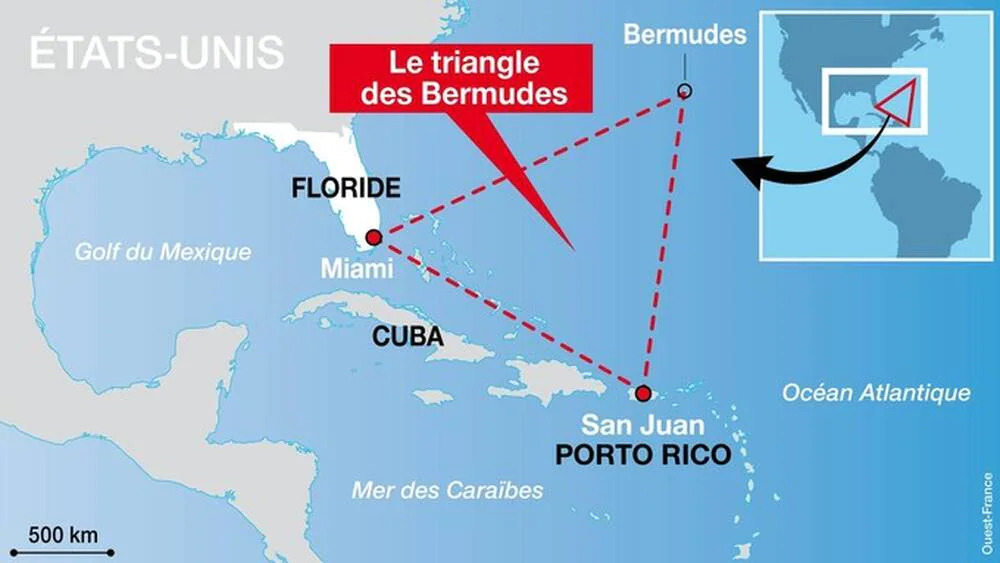
\includegraphics[scale=0.17]{bermudes.jpg}
        \end{center}
    \end{columns}
  \end{frame}

  \begin{frame}{Mort}
    \hypertarget{mort}{}
    \begin{columns}
      \column{0.5\textwidth}
        Tu te trouves au fond du casier de Davy Jones, mais il te prend en pitié.
        Il t'envoie \hyperlink{début}{à ton bateau}...
      \column{0.5\textwidth}
        \begin{center}
          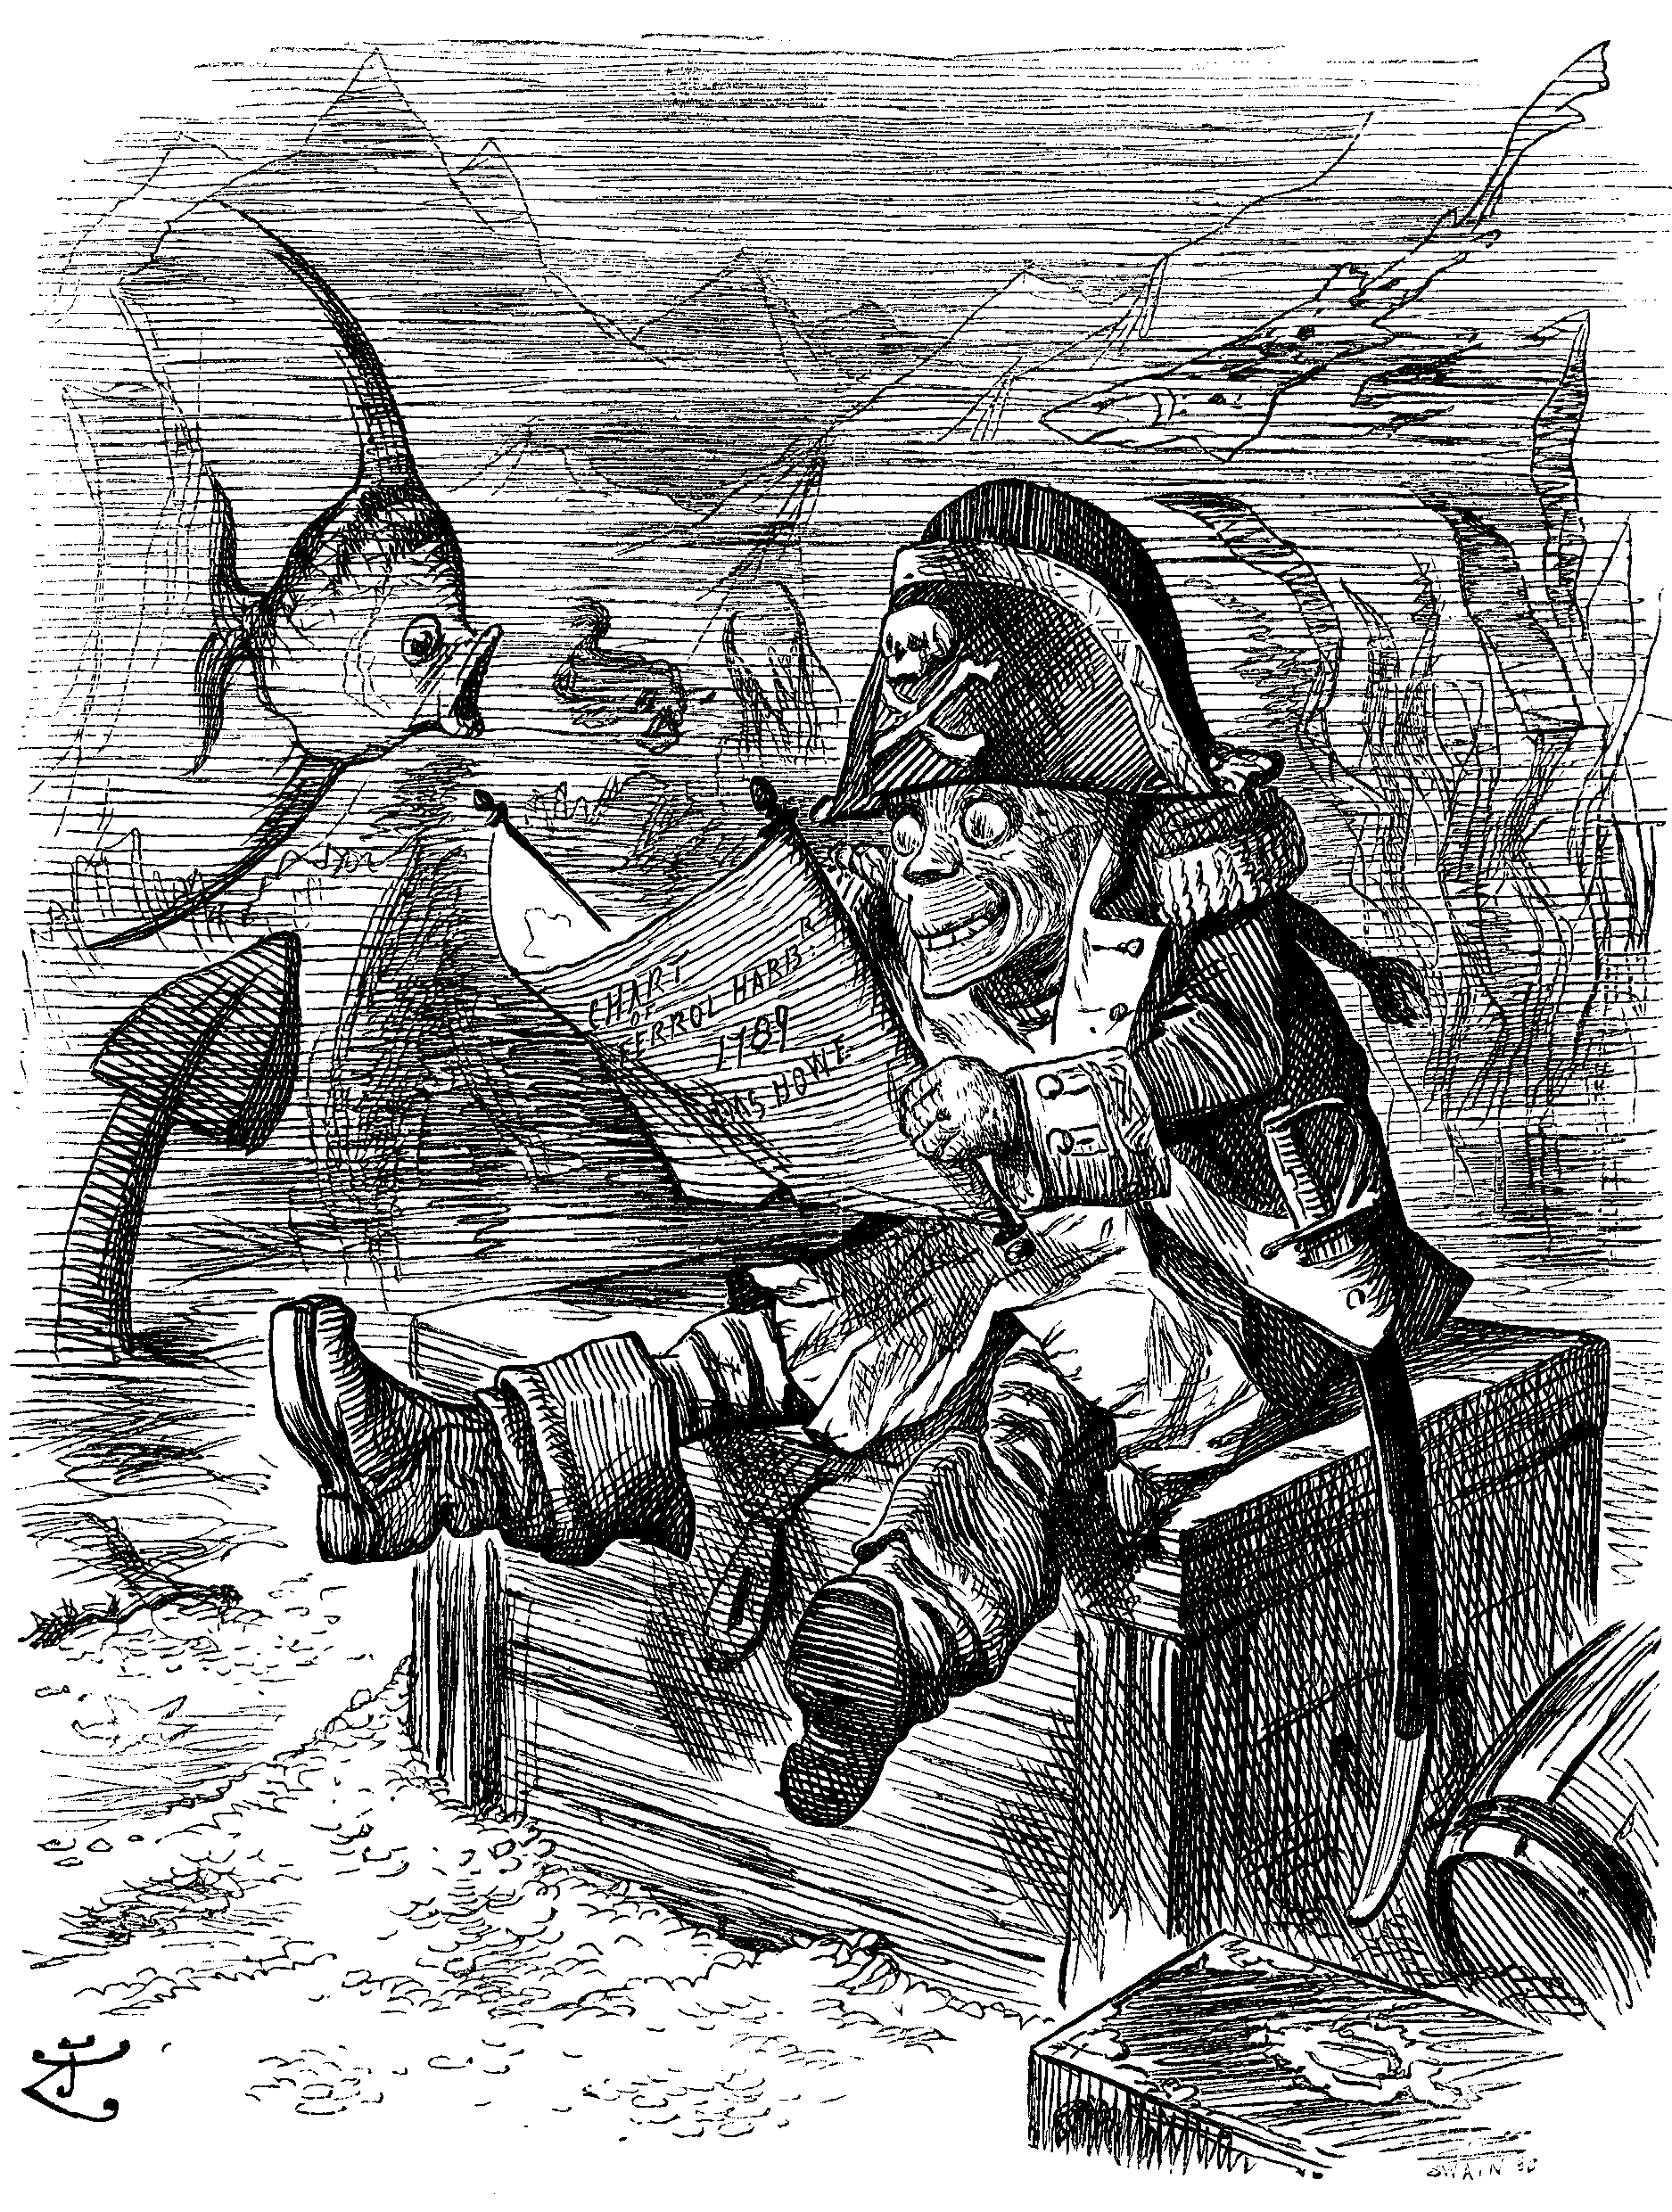
\includegraphics[scale=0.3]{casier.png}
        \end{center}
    \end{columns}
  \end{frame}
\end{document}